%
\section{Математическая модель}
%
В работе проводится моделирование трехфазной фильтрации несмешивающихся
жидкостей и газа с учетом их сжимаемости. Все протекающие процессы считаем
изотермическими, скелет породы -- неподвижным, пористость -- постоянной во всем
рассматриваемом объеме, среду -- изотропной, жидкие фазы -- слабосжимаемыми,
газ -- идеальным.

Класс решаемых задач включает в себя как двумерные, так и трехмерные 
прямоугольные области, координаты декартовы.

Рассматриваем трехфазную систему, такую что две фазы жидкие -- вода и легкий
нефтяной продукт(LNAPL -- от английского Light Non-Aqueous Phase Liquids, 
плотность меньше плотности воды), и одна газообразная.
Для удобства введем индексные обозначения для разных фаз: $w$ -- вода, $n$ --
легкая нефть, $g$ -- газ.
В трехфазной системе имеются 2 независимых насыщенности. Без ограничения
общности считаем, что это насыщенности воды и нефти. А насыщенность газа
будет определятся из соотношения: $S_g = 1 - S_w - S_n$.

Вводятся эффективные насыщенности каждой из фаз: 
$\overline{S_i}={\dfrac{S_i-S_{ir}}{1-S_{wr}-S_{nr}-S_{gr}}}$, где $S_{wr}$, 
$S_{nr}$, $S_{gr}$ -- остаточные насыщенности фаз.

Всего в системе три независимых переменных. В качестве третьей переменной берем
давление воды $P_w$. $P_n$ и $P_g$ отличаются от $P_w$ на величины капиллярных
давлений, являющихся функциями от насыщенностей. Для описания
капиллярных давлений выбрана приближенная модель Паркера:
$$P_{cnw}(S_w)=P_n-P_w={\frac{1}{\alpha \beta_{nw}}}\left( \overline{S_w}^{\frac{n}{1-n}}-1 \right)^\frac{1}{n},\;0<\overline{S_w}<1 $$
$$P_{cgn}(S_g)=P_g-P_n={\frac{1}{\alpha \beta_{gn}}}\left( (1-\overline{S_g})^{\frac{n}{1-n}}-1 \right)^\frac{1}{n},\;0<\overline{S_g}<1$$
(где $P_{cnw}(S_w)$ - и $P_{cgn}(S_g)$- капиллярные давления на границах вода-нефть и нефть-газ, 
соответственно, $n$ и $\alpha $ -- пареметры породы Ван Генухтена из соответствующего приближения
Ван Генухтена, $\beta_{nw}$, $\beta_{gn}$ -- коэффициенты, определяемые поверхностным натяжением 
жидкостей). В работе используются следующие значения параметров: $n$ = 3.25, $\alpha $ = 0.00048Па$^{-1}$,
$\beta_{nw}$ = 0.67, $\beta_{gn}$ = 2, $K=6.64\cdot 10^{-11}$ м$^2$, $m$=0.4. На участках, где эффективные насыщенности перестают удовлетворять
указанному интервалу, гладко продалжаем указанные функции капиллярных давлений. Изобразим полученные зависимости
на графиках:
\begin{center}
 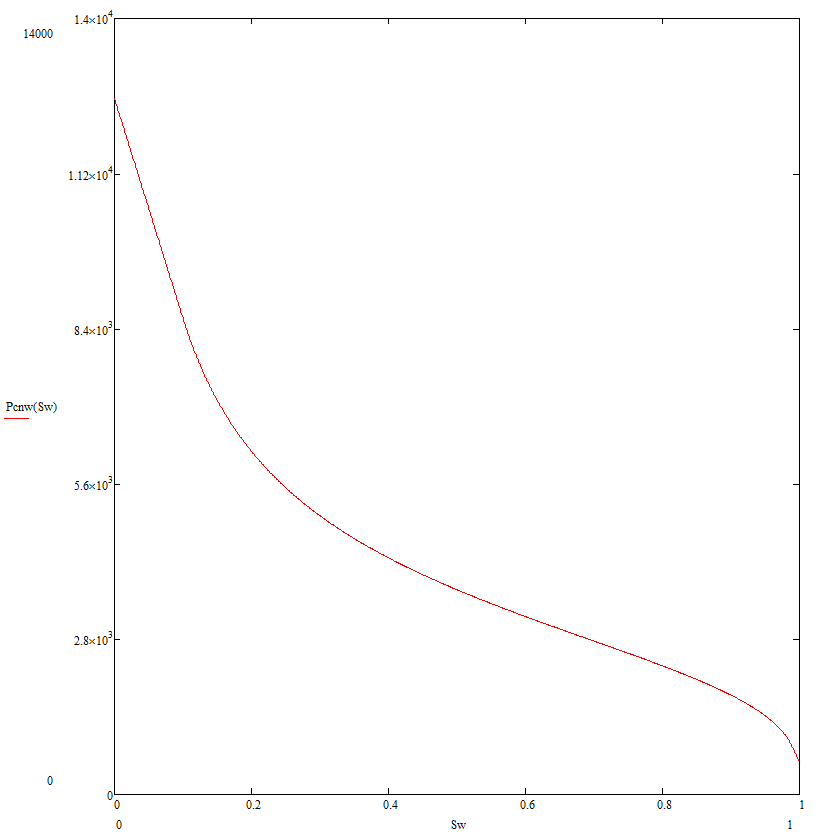
\includegraphics[width=7cm,height=9cm]{Pcnw}
 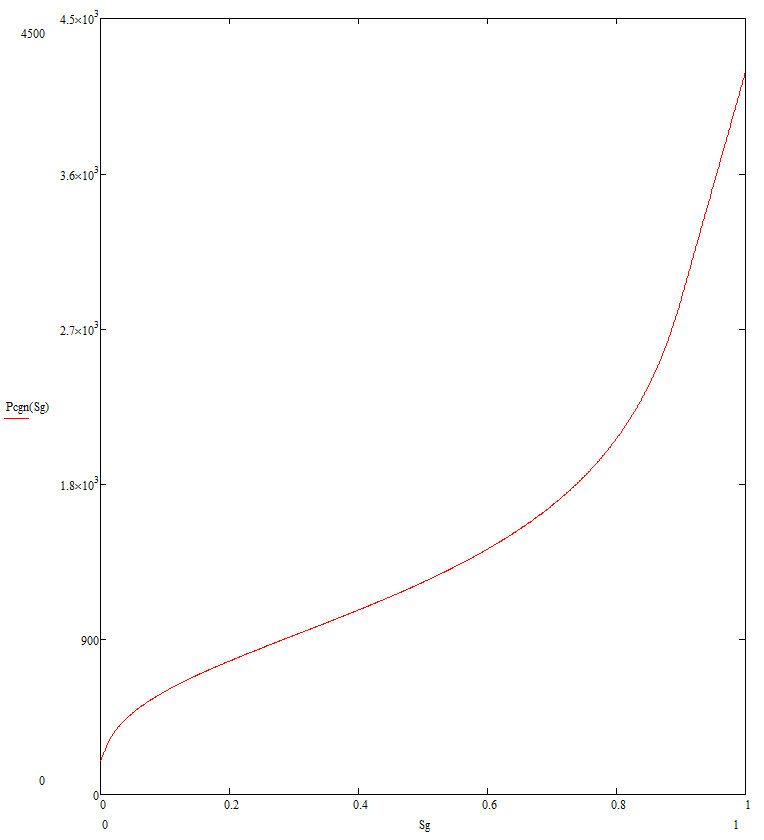
\includegraphics[width=7cm,height=9cm]{Pcgn}
\end{center}

Относительные фазовые проницаемости определяются в работе в соответствии с
приближением Стоуна в модификации Азиза и Сеттари:

\begin{equation*}
  k_{w}(S_w)=
  \begin{cases}
  &\overline{S_w}^\frac{1}{2} \left( 1-\left( 1-\overline{S_w}^\frac{n}{n-1} \right) ^\frac{n-1}{n} \right) ^2
  \text{ if $0<\overline{S_w}<1$}\\
  &1 \text{ if $\overline{S_w}\ge 1$}\\
  &0 \text{ if $\overline{S_w}\le 0$}
\end{cases} 
\end{equation*}
\begin{equation*}
  k_{g}(S_g)=
  \begin{cases}
  &\overline{S_g}^\frac{1}{2} \left( 1-\left ( 1-\overline{S_g} \right) ^\frac{n}{n-1} \right) ^\frac{2(n-1)}{n}
  \text{ if $0<\overline{S_g}<1$}\\
  &1 \text{ if $\overline{S_g}\ge 1$}\\
  &0 \text{ if $\overline{S_g}\le 0$}
  \end{cases} 
\end{equation*}
\begin{center}
 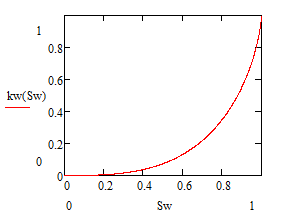
\includegraphics[width=7cm,height=6cm]{kw}
 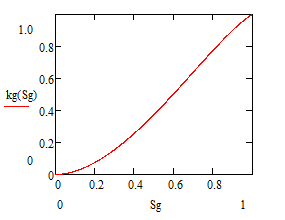
\includegraphics[width=7cm,height=6cm]{kg}
\end{center}
\begin{equation*}
  k_{n}(S_w,S_n)=
  \begin{cases}
  &\dfrac{\overline{S_n} k_{nw}(S_w)k_{ng}(S_n)}{(1-\overline{S_w})(\overline{S_w}+\overline{S_n})}
  \text{ if $\overline{S_w}<1, \quad \overline{S_w}+\overline{S_n} >0$}\\
  &0 \text{ otherwise}
  \end{cases}  
\end{equation*}
, \\
\text{где } 
\begin{equation*}
  k_{nw}(S_w)=
  \begin{cases}
  &(1-\overline{S_w})^\frac{1}{2} \left(1-\overline{S_w}^\frac{n}{n-1} \right) ^\frac{2(n-1)}{n}
  \text{ if $0<\overline{S_w}<1$}\\
  &1 \text{ if $\overline{S_w}\le 0$}\\
  &0 \text{ if $\overline{S_w}\ge 1$}
  \end{cases}
\end{equation*}
, \\
\begin{equation*}
  k_{ng}(S_n)=
  \begin{cases}
  &\overline{S_n}^\frac{1}{2} \left( 1-\left( 1-\overline{S_n}^\frac{n}{n-1} \right) ^\frac{n-1}{n} \right) ^2 
  \text{ if $0<\overline{S_n}<1$}\\
  &1 \text{ if $\overline{S_n}\ge 1$}\\
  &0 \text{ if $\overline{S_n}\le 0$}
\end{cases}\text{.} 
\end{equation*}
\begin{center}
 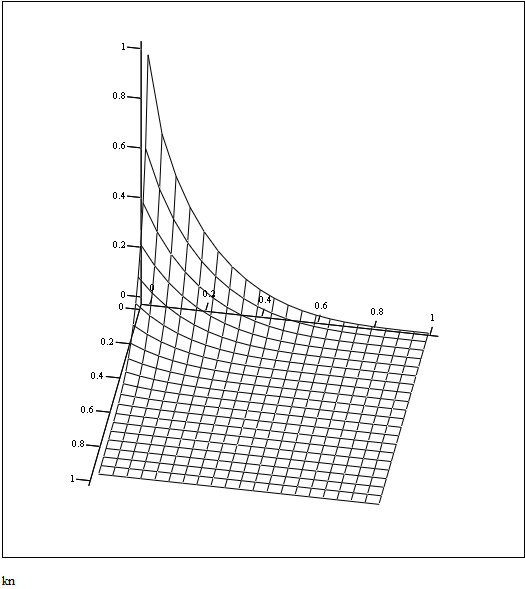
\includegraphics[width=12cm,height=12cm]{kn}
\end{center}
 
Таким образом, относительные проницаемости воды и газа являются функциями одной 
переменной(насыщенности одной
из фаз), а нефти -- двух.

Водную и нефтяную фазы считаем слабосжимаемыми:\\
$${\rho}_i = {\rho}_{i0} + {\beta}(P_i-P_0),{\quad}0<{\beta}{\ll}1,{\quad}i=w,n,$$
где ${\rho}_{i0}$ -- известное значение плотности $i$-ой фазы, соответсвующее
значению давления $P_0$.

Для газа предполагаем справедливым уравнение состояния идеального
газа(температура среды постоянна):
$${\rho}_g = {\rho}_{g0}{\frac{P_g}{P_0}}$$

Для всех трех фаз полагаем, что выполняется закон Дарси.

Таким образом, полная система уравнений для описания трехфазной системы
принимает вид:
\begin{equation}
\left\{
  \begin{aligned}
    &\overrightarrow{u_i}=-K \frac{k_i(S_i)}{{\mu}_i}(grad P_i - {\rho}_i\overrightarrow{g})\\
    &m\frac{\partial (\rho_i S_i)}{\partial t}+ div(\rho_i \overrightarrow{u_i}) = 0 \\
    &{\rho}_i = {\rho}_i(P_i) \\
    &i=w,n,g\\
    &P_n=P_w+P_{cnw}(S_w)\\
    &P_g=P_w+P_{cnw}(S_w)+P_{cgn}(S_g)\\
    &S_w + S_n + S_g=1
  \end{aligned}
\right.
\end{equation}

В зависимости от конкретной постановки задачи в работе используются различные
граничные условия.Для давления задаются условия непротекания (равны нормальные 
к границе области компоненты скорости) или условия поддержания на границе постоянного
давления. Для насыщенности ставится условие равенства нулю потока через граничную 
поверхность или же задается поток насыщенности в виде известной функции через 
$ \dfrac{\partial S_i}{\partial n_j}, \; i=w,n, \;  n_j \text{-- нормаль к $j$-ой границе} $.

В начальный момент времени считаем известными распределение давлений водной 
фазы и распределение насыщенностей по всей области.
